\chapter{Evaluation}

To measure the effectiveness of dynamic windowing for multi-stream operators during the 
mapping of non-RDF heterogeneous data, we would need to measure the following 
metrics of our stream processing framework: \emph{latency}, \emph{throughput},
\emph{memory usage} and \emph{completeness}. \emph{Throughput}, in this 
paper, refers to the number of output/processed records per time unit.
\gh{Does the slash mean "divided by", or "or", or something else? Avoid slashes outside formulas... Would it be accurate to say that throughput is the "number of processed input records per time unit"? "Input records" because some mappings produce no output records, and "processed" because they only count after processing them.} 
\emph{Latency, throughput,} and \emph{memory usage} can be measured following the recent benchmark studies by 
Van Dongen and Van den Poel(2020)~\cite{evalution_of_spe}.
However, to evaluate 
for the \emph{completeness/quality}
\gh{Same remark. Perhaps choose "completeness" to be consistent with the rest of the text. If you go for "quality", please explain very well what exactly that means.}
of the generated output, a reference output needs 
to be generated for comparison. Since a data stream is \sout{in principle} unbounded in nature, 
and cannot be processed completely to check for \emph{completeness}, a bounded 
dataset of relatively large volume \sout{could} will be used to measure \emph{completeness}.
To ensure consistency in the complexity of the multi-stream operator being used, 
we will apply the join operator in the windows --- a common operator used in 
data enrichment scenarios. 


The following sections will describe the methodology and the data used to evaluate the
different metrics. Setups required to reproduce the evaluation will also be elaborated 
in their respective sections. 


\section{Data}

Assessment of our dynamic windowing scheme for multi-stream operator will require 
the data to have some common attributes to enrich the data. Furthermore, to 
mirror a real-world scenario, we would also employ data gathered from IoT sensors
\sout{because of its common usage in data stream processing}.
\gh{I think mirroring a real-world scenario is more important than whether or not such data are used in stream processing.}
We will use the same data 
as is the case for the benchmark in the paper by Van Dongen and Van den Poel~\cite{evalution_of_spe}. 
\sout{To recap,} The data is provided by NDW (Nationale Databank Wegverkeersgegevens) from the 
Netherlands \gh{add url as footnote if publicly available}. It consists of measurements of the number of cars and their average speed. 
A subset of the complete sensor data will be replayed by a Kafka publisher into the two topics 
\emph{flow} and \emph{speed}, for the number of cars and the average speed respectively. 

\subsection{Data for completeness evaluation}
Completeness measure requires a dataset which could be mapped completely by a static 
mapping engine. RMLMapper \todo{maybe RMLStreamer for static set might be enough?}
\gh{Good question. In theory that would be enough since it should produce the same results as the RMLMapper. You could also say that the complete set of output triples is generated according to the RML spec (then the implementation doesn't really matter)}
will
be used to generate our \emph{complete} set of output triples. Streaming data is usually 
ordered according to the event time \gh{Make sure "event time" is defined somewhere. Maybe even in the chapter on stream processing?} and the same entity could appear in the 
stream at a different timestamp. This can lead to duplicates in the generated output by 
the RMLMapper. Therefore, duplicates in the generated output by the reference optimal
mapping engine needs to be removed in the final \emph{complete} output dataset.
\gh{In theory the output is an RDF graph, where duplicates don't count. But what with statements that are not duplicates? e.g. if we first have :It :is "day" and later on :It :is "night"? We can probably avoid this by incorporating the timestamp in the subject iri or generating quads where the graph holds a timestamp.}

\section{Evaluation pipeline}

\begin{figure}[!htbp]
    \centering
    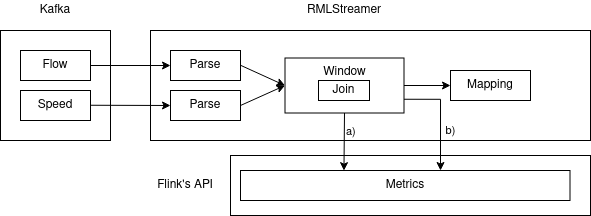
\includegraphics[width=\textwidth]{fig/evaluation_architecture.png}
    \caption{Evaluation flow based on~\cite{evalution_of_spe} with some changes to only 
    take metrics at the "Join" and the "Mapping" stage. a) \emph{throughput} of the generated output triple \gh{What do you mean by throughput of a triple? Do you mean nr of triples per second?}. 
    b) \emph{latency} of evaluating the join operator in windows.}
    \label{fig:evaluation_flow}
    
\end{figure}

Similar to the workflow process in~\cite{evalution_of_spe, benchmark_dsp}, we set up
our evaluation pipeline as illustrated in Figure~\ref{fig:evaluation_flow}. Setting it 
up according to the illustrated pipeline, allows us to have fine control over the 
workload scenarios and limit the measurement of the metrics just to the windows. 



\section{Workload scenarios}
As stated in Chapter~\ref{chap:data_stream_processing}, data streams have characteristics 
which determine the performance of stream processing frameworks and its operators. Therefore, 
there is a need to evaluate our dynamic window implementation under different workload scenarios. 

\subsection{Workload for maximum throughput measurement}
This workload will attempt to measure the maximum throughput RMLStreamer can 
process with the different windows, before \emph{latency,} and \emph{memory utilization}
increasing significantly. We will increase the velocity of the input data gradually 
every 10 seconds until there is a significant latency of more than 10 seconds to produce
the next output triple or until the memory allocated to the instances get fully used up. 


\subsection{Workload for latency measurement}



\subsection{Workload for failure restart}


\subsection{Workload for completeness}

\subsection{Workload with increasing burst }

\subsection{Workload with periodic burst}


\section{Environment}




